\canonabc{} generates a complete canon\footnote{In music, a canon is a contrapuntal compositional
technique that employs a melody with one or more imitations of the melody played after a given
duration. It is possible for a canon to be accompanied by one or more additional independent parts
which do not take part in imitating the melody.} score from a set of \abc{} files containing the
melodic part and other file containing the accompaniment part. The order in which the \abc{} files
are provided to \canonabc{} is important as they determine the voices' order in the final score.

The only part in a canon's form that is not simple to automate is the canon's finale, as it depends
on the composer's will and taste. So that part is left for the composer to change manually.

In \canonabc, the base duration, after which another voice may start playing, is a full measure.
Thus, in this section, that duration is treated in \measurerests{}.

The melodic part is played by as many voices as the user specifies and each one of them may start at
different time offsets (specified by the user in number of \measurerests{}). The accompaniment part
is repeated until it has the same number of measures as the melodic parts.

\canonabc{} requires the user to provide the number of \measurerests{} each melodic part should have
at the beginning as well as identify which \abc{} file is the accompaniment part. This is achieved
through a slight modification on the arguments that \canonabc{} is expecting. So, in order to meet
the first requisite, the user must append to each melody file the string \emph{+Num} (where
\emph{Num} is the number of \measurerests{} to insert at the beginning) and to meet the second
requisite he must append the string \emph{++}.

This tool reuses other \abcpt{}s (\catabc{} and \pasteabc{}) in order to accomplish some of the
features proposed.

\subsection*{Algorithm}

\canonabc{}'s algorithm consists of 3 stages: \textbf{1)} extract information from \canonabc{}'s
arguments, \textbf{2)} build the canon's melodic parts and \textbf{3)} build the canon's
accompaniment part. In the end, the generated score is printed to the output.

An algorithmic description is made in algorithm \ref{alg:canonabc}.\\

\begin{enumerate}
  \item Extract information from \canonabc{}'s arguments about the parts of the canon.

  In this stage, for each melodic part, the file name and the number of \measurerests{} are stored.
  For the accompaniment part the file name is stored.

  \item Build the canon's melodic parts

    For each melodic part and its information:
    \begin{enumerate}
      \item Add \measurerests{} at the beginning

      The \abcpt{} \catabc{} is used to achieve this by using the option \emph{-d}.

      \item Add voice header

      This consists of processing the part (\abc{} tune) with \dt{} in order to add a single new
      voice header (e.g.: \emph{V:1}). The set of \abcdt{} rules is shown in table
      \ref{tab:canon_add_voice_rules}.

      \begin{center}
        \begin{table}[h]
          \begin{tabular}{|p{2.5cm}|p{4.75cm}|p{8cm}|}
            \hline
            Actuator & Transformation (Perl) & Notes\\
            \hline
            \hline
            \emph{in\_header::K:} & add\_voice\_header(); & Local function that appends a voice header
            after the key definition.
            \\
            \hline
          \end{tabular}
          \caption{\abcdtrules{} for \canonabc{}'s stage 2-b)}
          \label{tab:canon_add_voice_rules}
        \end{table}
      \end{center}
    \end{enumerate}
    At the end of this stage, all melodic parts are merged into one single score, here called of
    \emph{melody}. This is achieved with \pasteabc{}.

  \item Build the canon's accompaniment part

    \begin{enumerate}
      \item Add voice header to the accompaniment part and count measures

      This consists of processing the accompaniment part (\abc{} tune) with \dt{} in order to add a new voice
      header (e.g.: \emph{V:1}) and count the number of measures. The set of \abcdt{} rules is shown
      in table \ref{tab:canon_add_voice_and_count_measures_rules}.

      \begin{center}
        \begin{table}[h]
          \begin{tabular}{|p{2.5cm}|p{4.75cm}|p{8cm}|}
            \hline
            Actuator & Transformation (Perl) & Notes\\
            \hline
            \hline
            \emph{in\_header::K:} & add\_voice\_header(); & Local function that appends a voice header
            to the key definition.
            \\
            \hline

            \hline
            \emph{bar} & update\_measure\_count(); & Local function that updates the measure count
            \\
            \hline
          \end{tabular}
          \caption{\abcdtrules{} for \canonabc{}'s stage 3-a)}
          \label{tab:canon_add_voice_and_count_measures_rules}
        \end{table}
      \end{center}

      \item Count measures of \emph{melody}

      The number of measures in \emph{melody} is counted. The set of \abcdt{} rules is shown in
      table \ref{tab:canon_count_measures_rules}.

      \begin{center}
        \begin{table}[h]
          \begin{tabular}{|p{2.5cm}|p{4.75cm}|p{8cm}|}
            \hline
            Actuator & Transformation (Perl) & Notes\\
            \hline
            \hline
            \emph{bar} & update\_measure\_count(); & Local function that updates the measure count
            \\
            \hline
          \end{tabular}
          \caption{\abcdtrules{} for \canonabc{}'s stage 3-b)}
          \label{tab:canon_count_measures_rules}
        \end{table}
      \end{center}


      \item Repeat the accompaniment part

      In this step, the number of times the accompaniment part will be repeated is calculated by
      dividing \emph{melody}'s number of measures by the accompaniment part's number of measures.

      Then, the accompaniment part is repeated using \catabc{} with option \emph{-r}.

      \item Merge melody and accompaniment

      The final step consists in merging the melodic and accompaniment parts to form the canon. This
      is achieved through \pasteabc{}.
    \end{enumerate}
\end{enumerate}

\begin{algorithm}[h]
  \KwIn{args}
  $canon\_info \gets extract\_canon\_info(args)$ \hfill //1)\\
  \ForAll{$ melody \in canon\_info\{melodic\_parts\} $}{
    $m1 \gets cat\_abc$ -$d$=$melody\{delta\}$ $melody\{file\}$ \hfill //2-a)\\
    $m2 \gets dt(m1,$ rules from table \ref{tab:canon_add_voice_rules}$)$ \hfill //2-b)\\
  }
  $mel \gets paste\_abc $ (* for every $m2$ *) \hfill //2)\\

  $(acc, acc\_meas) \gets dt(canon\_info\{accomp\_part\},$ rules from table \ref{tab:canon_add_voice_and_count_measures_rules}$)$ \hfill //3-a)\\
  $mel\_meas \gets dt(res,$ rules from table \ref{tab:canon_count_measures_rules}$)$ \hfill //3-b)\\
  $acc\_reps \gets calculate\_reps(mel\_meas, acc\_meas)$ \hfill //3-c)\\
  $acc \gets cat\_abc$ -$r$=$acc\_reps$ $acc$ \hfill //3-c)\\
  $res \gets paste\_abc$ $mel$ $acc$ \hfill //3-d)\\
  \Return{$res$}
  \caption{\canonabc{}'s algorithm}
  \label{alg:canonabc}
\end{algorithm}

\subsection*{Usage}

Listing \ref{lst:canonabcman} shows \canonabc{}'s manual.\\

\lstinputlisting[caption={\canonabc{}'s manual},label={lst:canonabcman},captionpos=t,abovecaptionskip=-\medskipamount]{misc/canon_manual.tex}


Listing \ref{lst:canonabcbyexample} shows a usage example for \canonabc{}. It reads the melody files
\textbf{violini.abc} (appendix \ref{sec:pcanon_melody}) along with the respective number of
\measurerests{} and the accompaniment file \textbf{basso.abc} (appendix \ref{sec:pcanon_accomp}).
The output is shown in appendix \ref{sec:pcanon} and figure \ref{fig:pcanon_scheme} illustrates the
output's scheme.\\

\begin{lstlisting}[caption={\canonabc{} by example},label={lst:canonabcbyexample},captionpos=t,abovecaptionskip=-\medskipamount]
canon_abc violini.abc+8 violini.abc+16 violini.abc+24 basso.abc++
\end{lstlisting}

\begin{figure}[H]
  \begin{center}
    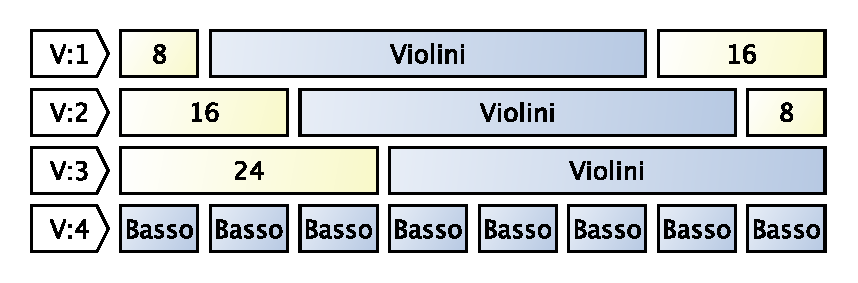
\includegraphics[width=0.8\textwidth]{img/pcanon_scheme.pdf}
    \caption{\canonabc{}'s output scheme}
    \label{fig:pcanon_scheme}
  \end{center}
\end{figure}
